\input{preamble/preamble_twocol.tex}
\input{preamble/definitions.tex}

\setlist[itemize]{leftmargin=*,itemindent=0pt,label=\textcolor{Col1}{\tiny$\blacksquare$}}
\setlist[enumerate]{leftmargin=*,itemindent=0pt,label=\textcolor{Col1}{\theenumi.}}

\setlength{\columnseprule}{1pt}
\setlength{\columnsep}{10mm}
\def\columnseprulecolor{\color{Col1}}


\begin{document}
\pagestyle{vangelis}

\begin{center}
    \large\bfseries\textcolor{Col2}{Πραγματικοί Αριθμοί} \\
    \large\bfseries\textcolor{Col2}{(Λύσεις των Ασκήσεων)}
\end{center}

\vspace{\baselineskip}



\begin{multicols}{2}

    \begin{enumerate}
        \setcounter{enumi}{1}

    \item \textcolor{Col1}{Για τα παρακάτω σύνολα, να υπολογιστούν και να αποδειχθούν τα 
        supremum και infimum.}


        \begin{enumerate}[i)]
            \item {\boldmath\textcolor{Col2}{$A = (0,2) $}}. 
                \begin{proof}
                \item {}

                    Έχουμε ότι $ \sup A = 2 $ και $ \inf A = 0 $.
                    \begin{itemize}
                        \item Θα δείξουμε ότι $ \sup A = 2 $. Πράγματι:

                            $2$ α.φ. του $A$, γιατί $ a < 2, \; \forall a \in A $.

                            Έστω $M$ α.φ. του $A$, δηλ. $a \leq M, \; \forall a \in A $.

                            Θ.δ.ο. $ 2 \leq M $ (Με άτοπο). Πράγματι:

                            Έστω $ M < 2 $. Τότε $ (M,2) \neq \emptyset $, άρα 
                            $ \exists a \in (M,2) $.

                            Όμως $ a \in A $ με $ a < 2 $. 
                            άτοπο, γιατί $ 2 $ α.φ. του $A$.

                        \item Θα δείξουμε ότι $ \inf A = 0 $. Πράγματι:

                            $0$ κ.φ. του $A$, γιατί $ a > 0, \; \forall a \in A $.

                            Έστω $m$ κ.φ. του $A$, δηλ. $a \geq m, \; \forall a \in A $.

                            Θ.δ.ο. $ 0 \geq m $ (Με άτοπο). Πράγματι:

                            Έστω $ m > 0 $. Τότε $ (0,m) \neq \emptyset $, άρα 
                            $ \exists a \in (0,m) $. 

                            Όμως $ a \in A $ με $ a > 0 $, 
                            άτοπο, γιατί $ 0 $ κ.φ. του $A$.
                    \end{itemize}
                \end{proof}

            \item {\boldmath\textcolor{Col2}{$ A = \{ x \in \mathbb{R} \; 
                : \; x < 0 \} $}}. 

                \begin{proof}
                \item {}

                    Έχουμε ότι $ \sup A = 0 $ και $ \inf A = - \infty $.
                    \begin{itemize}
                        \item Θα δείξουμε ότι $ \sup A = 0 $. Πράγματι:

                            $ 0 $ α.φ. του $A$, γιατί $ a < 0, \; \forall a \in A $.

                            Έστω $M$ α.φ. του $A$, δηλ. $a \leq M, \; \forall a \in A $.

                            Θ.δ.ο. $ 0 \leq M $ (Με άτοπο). Πράγματι:

                            Έστω $ M < 0 $. Τότε $ (M,0) \neq \emptyset $, άρα 
                            $ \exists a \in (M,0) $.

                            Όμως $ a \in A $ με $ a < 0 $, 
                            άτοπο, γιατί $ 0 $ α.φ. του $A$.

                        \item Θα δείξουμε ότι $ \inf A = -\infty $. Πράγματι:

                            $ A \neq \emptyset $ και $A$ όχι κάτω φραγμένο. Άρα 
                            $ \inf A = - \infty $.
                    \end{itemize}
                \end{proof}

            \item {\boldmath \textcolor{Col2}{$ A = \left\{ \frac{1}{n} \; 
                : \; n \in \mathbb{N} \right\} $}}.

                \begin{proof}
                \item {}

                    Έχουμε ότι $ \sup A = 1 $ και $ \inf A = 0 $.
                    \begin{itemize}
                        \item Θα δείξουμε ότι $ \sup A = 1 $. Πράγματι:

                            $ a \leq 1, \; \forall a \in A  $ και $ 1 \in A $ (για 
                            $ n=1 $). 

                            Άρα $ 1 = \max A $. Άρα $ \sup A = \max A = 1 $.

                        \item Θα δείξουμε ότι $ \inf A = 0 $. Πράγματι:

                            Προφανώς $ 0 \leq \frac{1}{n}, \; \forall n \in \mathbb{N} $, 
                            άρα το $ 0 $ κ.φ. του $A$.


                            Έστω $ \varepsilon > 0 $. Τότε $ \exists n_{0} \in \mathbb{N} $
                            με $ \frac{1}{n_{0}} < \varepsilon $ τ.ω. $ \frac{1}{n_{0}} 
                            < 0 + \varepsilon$, με $ \frac{1}{n_{0}} \in A $.
                    \end{itemize}
                \end{proof}

            \item {\boldmath \textcolor{Col2}{$ A = \left\{ \frac{n}{n+1} \; 
                : \; n \in \mathbb{N} \right\} $ }}

                \begin{proof}
                \item {}

                    Έχουμε ότι $ \sup A = 1 $ και $ \inf A = \frac{1}{2} $
                    \begin{itemize}
                        \item Θα δείξουμε οτι $ \sup A = 1 $

                            $ 1 $ α.φ. του $A$, γιατί $ \frac{n}{n+1} < 1, \; \forall n \in 
                            \mathbb{N}$.

                            (Δοκιμή: $ 1- \varepsilon < \frac{n}{n+1} \Leftrightarrow 
                            \varepsilon > 1 - \frac{n}{n+1} \Leftrightarrow \frac{1}{n+1} 
                            < \varepsilon \Leftrightarrow n+1 > \frac{1}{\varepsilon} 
                            \Leftrightarrow n > \frac{1}{\varepsilon} -1$ )

                            Έστω $ \varepsilon > 0 $. Τότε $ \exists n_{0} \in \mathbb{N}  $ με 
                            $ n_{0} > \frac{1}{\varepsilon} - 1 $ τ.ω. $ 1 - \varepsilon < 
                            \frac{n_{0}}{n_{0}+1}$, με $ \frac{n_{0}}{n_{0} +1} \in A $.

                        \item Θα δείξουμε ότι $ \inf A = \frac{1}{2} $. Πράγματι:

                            $ \frac{n}{n+1}  \geq \frac{1}{2}, \; \forall n \in \mathbb{N}  $
                            και $ \frac{1}{2} \in A$ (για $ n = 1 $).

                            Άρα $ \frac{1}{2} = \min A $. Άρα $ \inf A = \min A = \frac{1}{2} $.
                    \end{itemize}
                \end{proof}

            \item {\boldmath \textcolor{Col2}{$ A = \left\{ \frac{1}{n} + (-1)^{n} \; 
                : \; n \in \mathbb{N} \right\} $}}.

                \begin{proof}
                \item {}

                    Παρατηρούμε ότι \begin{align*} 
                        A &= \{ 0, \frac{1}{2} + 1, \frac{1}{3} -1, 
                        \frac{1}{4} + 1, \frac{1}{5} -1, \ldots  \} \\ 
                          &= \{ \frac{1}{2} + 1, \frac{1}{4} + 1, \ldots \} \cup 
                          \{ 0, \frac{1}{3} -1, \frac{1}{5} -1, \ldots \}  \\ 
                          &= \{ \frac{1}{2n} + 1 \; : \; n \in \mathbb{N}\} \cup 
                          \{ \frac{1}{2n-1} - 1 \; : \; n \in \mathbb{N}\} \\
                          &= A_{1} \cup A_{2} 
                        \end{align*}

                        Επίσης, έχουμε ότι:
                        $Α = \{ 0, \frac{3}{2}, -\frac{2}{3}, \frac{5}{4}, 
                        -\frac{4}{5}, \ldots \} $.

                        Αν παραστήσουμε τα στοιχεία του $A$, πάνω στην ευθεία των πραγματικών 
                        αριθμών, έχουμε:

                        \[
                            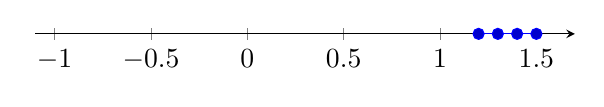
\begin{tikzpicture}
                                \begin{axis}[
                                    % center the x axis
                                    axis x line=middle,
                                    % we don't need a y axis line ...
                                    axis y line=none,
                                    % ... and thus there is no need for much `height' of the axis
                                    height=50pt,
                                    % but `height' also changes `width' which is restored here
                                    width=\axisdefaultwidth,
                                    xmin=-1.1,
                                    xmax= 1.7,
                                    ]
                                    \addplot coordinates {
                                            (1.2,0) (1.3,0) (1.4,0) (1.5,0) 
                                        };
                                \end{axis}
                            \end{tikzpicture}
                        \]

                        Παρατηρούμε ότι $ \inf A_{1} = 1 $ και $ \sup A_{1} = \max A_{1} = 
                        1+ \frac{1}{2} = \frac{3}{2} $.
                        Επίσης $ \inf A_{2} = -2 $ και $ \sup A_{2} = \max A_{2} = 0 $. 

                        Τότε, από γνωστή πρόταση θα έχουμε ότι $ \sup A = \max \{ \sup A_{1}, 
                        \sup A_{2}\} = \max \{ 0, \frac{3}{2} \} = \frac{3}{2}  $ και 
                        $ \inf A = \min \{ \inf A_{1}, \inf A_{2} \} = \min \{ -1, 1 \} = -1 $ 


                        Οπότε αρκεί να αποδείξουμε ότι $ \inf A_{1} = -1 $ και $ \sup A_{2} = 
                        \frac{3}{2} $. Πράγματι:

                        \begin{itemize}
                            \item Θα δείξουμε ότι $ \sup A_{2} = \frac{3}{2} $. Πράγματι:

                                $ \frac{3}{2} $ α.φ. του $A_{2} $, γιατί $ \frac{1}{n} + (-1)^{n} 
                                \leq \frac{3}{2}, \; \forall n \in \mathbb{N} $ 
                                και $ \frac{3}{2} \in A $. 

                                Άρα $ \frac{3}{2} = \max A_{2} $. Άρα $ \sup A_{2} = \max A_{2} 
                                = \frac{3}{2} $.

                            \item Θα δείξουμε ότι $ \inf A = -1 $. Πράγματι:

                                $ -1 $ κ.φ. του $A$, γιατί $ \frac{1}{n} + (-1)^{n} > -1, \; 
                                \forall n \in \mathbb{N} $.

                                (Δοκιμή: $ \frac{1}{2 n -1} -1 < -1 + \varepsilon 
                                \Leftrightarrow \frac{1}{2 n -1} < \varepsilon $,
                                το οποίο ισχύει, γιατί $ \frac{1}{2 n -1} < \frac{1}{n}, \forall 
                                n \in \mathbb{N} $).

                                Έστω $ \varepsilon > 0 $. Τότε $ \exists n_{0} \in \mathbb{N}  $ 
                                με $ \frac{1}{n_{0}} < \varepsilon $ τ.ω. $ \frac{1}{2 n_{0} -1} 
                                - 1 < \varepsilon -1 $, με $ \frac{1}{2 n_{0}} - 1 \in A $.
                        \end{itemize}
                    \end{proof}

                \item {\boldmath \textcolor{Col2} {$ A = \left\{ \frac{1}{n} - \frac{1}{m} \; : \; n,m \in 
                    \mathbb{N} \right\}$ }}

            Έχουμε ότι $ \sup A = 1 $  και $\inf A = -1 $.

            \begin{itemize}
                \item Θα δείξουμε ότι $ \inf A = -1 $. Πράγματι:

                    $ -1 $ κ.φ. του $A$, γιατί $ \frac{1}{n} - \frac{1}{m} \geq \frac{1}{n} 
                    - 1 > -1, \; \forall n \in \mathbb{N} $.

                    ΄
                    Εστω $ \varepsilon > 0 $. Τότε, $ \exists n_{0} \in \mathbb{N} $ με 
                    $ \frac{1}{n_{0} -1} < \varepsilon -1 - -1 + \varepsilon   $ με 
                    $ \frac{1}{n_{0} - 1} \in A $.

                \item Θα δείξουμε ότι $ \sup A = 1 $. Πράγματι:

                    Παρατηρούμε ότι $ A = -A $, άρα από γνωστή πρόταση έχουμε ότι 
                    \[ \inf A = - \sup (-A) = - \sup A \]
                    Άρα \[ \sup A = - \inf A = -(-1) = 1 \]
            \end{itemize}

            \end{enumerate}

        \pagebreak

        \item \textcolor{Col1}{Έστω $A$ φραγμένο υποσύνολο του $ \mathbb{R} $ τέτοιω ώστε $ \sup A = \inf A $.
            Να δείξετε ότι το $A$ είναι μονοσύνολο.}

            \begin{proof}
            \item {}
                Έστω $ c = \inf A = \sup A $. Τότε $ \forall a \in A $ ισχύει $ c \leq a \leq c
                $. Άρα $ A = \{ c \} $.
            \end{proof}

        \item \textcolor{Col1}{Αν $ A, B $ μη-κενά, φραγμένα υποσύνολα του $ \mathbb{R} $ με $ A \subseteq B $ να δείξετε ότι $ \inf B \leq \inf A \leq \sup A \leq \sup B $.}

            \begin{proof}
            \item {} 
                \begin{itemize}
                    \item Θα δείξουμε ότι $ \inf B \leq \inf A $. 

                        Αρκεί να δείξουμε ότι $ \inf B $ κ.φ. του $A$. Πράγματι:

                        Έστω $ x \in A \overset{A \subseteq B}{\Rightarrow} x \in B \Rightarrow 
                        \inf B \leq x, \; \forall x \in A $. Άρα $ \inf B $ κ.φ. του $A$.

                    \item Προφανώς $ \inf A \leq \sup A $, γιατί $ \forall x \in A, \; 
                        \inf A \leq x \leq \sup A $.

                    \item Θα δείξουμε οτι $ \sup A \leq \sup B $. 

                        Άρκεί να δείξουμε ότι $ \sup B $ α.φ. του $A$. Πράγματι:

                        Έστω $ x \in A \overset{A \subseteq B}{\Rightarrow} x \in B \Rightarrow 
                        x \leq \sup B, \; \forall x \in A $.  Άρα $ \sup B $ α.φ. του $A$.
                \end{itemize}
            \end{proof}

        \item \textcolor{Col1}{Έστω $ A, B $ μη-κενά υποσύνολα του $ \mathbb{R} $ τέτοια ώστε 
                $ a \leq b, \; \forall a \in A $ και $ \forall b \in B $.
                Να δείξετε ότι:
                \begin{enumerate}[i)]
                    \item $ \sup A \leq b, \;  \forall b \in B $
                    \item $ \sup A \leq \inf B $
            \end{enumerate}}

            \begin{proof}
            \item {}
                \begin{enumerate}[i)]
                    \item \label{prop:one} Έστω $ b \in B \Rightarrow a \leq b, \; 
                        \forall a \in A $. 
                        Άρα $ b \in B $ α.φ. του $A, \; \forall b \in B$. Άρα 
                        $ \sup A \leq b, \; \forall b \in B $.

                    \item Από το \ref{prop:one} έχουμε ότι $ \sup A \leq b, \; \forall 
                        b \in B$. Άρα το $ \sup A $ κ.φ. του $B$. Άρα $ \sup A \leq 
                        \inf B$.
                \end{enumerate}
            \end{proof}

        \item \textcolor{Col1}{ Έστω $ A \subseteq \mathbb{R} $ μη-κενό, και κάτω φραγμένο και έστω 
                $ B $ το σύνολο των κάτω φραγμάτων του $A$. Να δείξετε ότι:
                \begin{enumerate}[i)]
                    \item $ B \neq \emptyset $
                    \item $B$ άνω φραγμένο.
                    \item $ \sup B = \inf A $
            \end{enumerate}}

            \begin{proof}
            \item {}
                \begin{enumerate}[i)]
                    \item $A$ κάτω φραγμένο. Άρα $ \exists x \in \mathbb{R} $ τ.ω. $x$ 
                        κ.φ. του $A$, οπότε $ x \in B \Rightarrow B \neq \emptyset $.

                    \item $ A \neq \emptyset $, άρα $ \exists x \in A $. Τότε $ \forall 
                        y \in \mathbb{R}$ με $ y>x $ έχουμε ότι $ y $ όχι κ.φ. του A. 
                        Άρα $ y \not\in b $. Άρα το $ B $ είναι άνω φραγμένο.

                    \item 
                        $  
                        \left.
                            \begin{tabular}{l}
                                $ B \neq \emptyset $ \\
                                $B$ άνω φραγμένο
                            \end{tabular}
                        \right\}
                        \overset{\text{Α.Π.}}{\Rightarrow} B $ έχει supremum, έστω $ a = \sup B $.
                        Τότε $ a \geq x, \; \forall x \in B $, άρα $ a \geq x, \; \forall x $
                        όπου $x$ είναι κ.φ. του $A$, άρα $ a \geq \inf A $. Οπότε αρκεί να 
                        δείξουμε ότι $ \inf A \geq a $, δηλ. αρκεί να δείξουμε ότι $ 
                        a$ κ.φ. του $A$ (Με άτοπο). Πράγματι:

                        Έστω ότι $ a $ όχι κ.φ. του $A$. Άρα $ \exists x \in A, \; x < a $. 
                        Όμως $ a = \sup B $, οπότε από τη χαρ. ιδιοτ. του supremum έχουμε ότι
                        $ \exists y \in B, \; x < y < a $. Άτοπο, γιατί $ y $ κ.φ. του $A$.

                        Άρα $ \sup B = \inf A $.

                \end{enumerate}
            \end{proof}


        \item \textcolor{Col1}{\label{ask:3z} Να αποδείξετε ότι το σύνολο $ A 
            = \{ 3k \; : \; k \in \mathbb{Z} \} $ δεν είναι άνω φραγμένο.}

            \begin{proof}
            \item {}
                Πράγματι, έστω $ A $ άνω φραγμένο, και επειδή $A \neq \emptyset $ 
                υπάρχει το supremum του $A$, έστω $ \sup A = s $. Τότε $ s-1 < s $.
                Άρα από τη χαρ. ιδιοτ. του supremum, $ \exists k \in \mathbb{Z}, \; 
                3k > s-1$. Άρα $ 3k+3 > s-1 + 3 \Leftrightarrow 3(k+1) > s+2 > s $. Όμως 
                $ 3(k+1) \in \mathbb{Z} $, άτοπο, γιατί $ s = \sup A $.
            \end{proof}

        \item \textcolor{Col1}{Έστω $ A,B $ μη-κενά, φραγμένα υποσύνολα του $ \mathbb{R} $.
                Να δείξετε ότι:
                \begin{enumerate}[i)]
                    \item $ A \cup B  $ είναι φραγμένο
                    \item $ \sup {(A\cup B)} = \max \{ \sup A, \sup B \} $
                    \item $ \inf {(A\cup B)} = \min \{ \inf A, \inf B \} $
                    \item Ισχύει κάτι ανάλογο για το $ \sup {(A\cap B)} $ και 
                        $ \inf {(A\cap B)} $;
            \end{enumerate}}

            \begin{proof}
            \item {}
                \begin{enumerate}[i)]
                    \item {}
                        $A$ φραγμένο $ \Leftrightarrow \exists M \in \mathbb{R} 
                        > 0, \; -M < a < M, \; \forall a \in A $ 

                        $B$ φραγμένο $ \Leftrightarrow \exists N \in \mathbb{R} 
                        > 0, \; -N < b < N, \; \forall b \in B $ 

                        Θέτουμε $ K = \max \{ M,N \} $. 

                        Θα αποδείξουμε (με άτοπο) ότι $ -K < c < K, \; 
                        \forall c \in A \cup B $.Πράγματι:

                        Έστω $ c \in A \cup B $ με $ \abs{c} \geq K = \max \{ 
                        M,N\} $. Τότε 

                        $ 
                        \left.
                            \begin{tabular}{l}
                                Αν $c \in A$ τότε $M > \abs{c} \geq \max \{ M,N \}$, 
                                άτοπο \\
                                Αν $c \in B$ τότε $N > \abs{c} \geq \max \{ M,N \}$,
                                άτοπο
                            \end{tabular} 
                        \right\}  \Rightarrow -K < c < K, \; \forall c \in A \cup B $.


                    \item 
                        $
                        \left.
                            \begin{tabular}{l}
                                $ A \neq \emptyset $, και άνω φραγμένο $
                                \overset{\text{Α.Π.}}{\Rightarrow} \exists \sup A  $ \\

                                $ B \neq \emptyset $, και άνω φραγμένο $
                                \overset{\text{Α.Π.}}{\Rightarrow} \exists \sup B  $ \\
                            \end{tabular}
                        \right\}  \Rightarrow $ χ.β.γ. έστω $ \max \{ \sup A, \sup B \} = 
                        \sup A$. 

                        Θα δείξουμε ότι $ \sup (A \cup B) = \sup A $. Πράγματι:

                        Έστω $ c \in A \cup B $. Τότε, αν $ c \in A \Rightarrow c \leq 
                        \sup A$, ενώ αν $ c \in B \Rightarrow c \leq \sup B \leq \sup A $. 
                        Άρα σε κάθε περίπτωση $ c \leq \sup A, \; \forall c \in A \cup 
                        B$. Άρα $ \sup A $ α.φ. του $ A \cup B $.

                        Ισχύει ότι \inlineequation[eq:first]{ \sup (A \cup B) 
                        \leq \sup A }, γιατί $ \sup A $ α.φ. 
                        του $ A \cup B $. Θα δείξουμε ότι \inlineequation[eq:two]{ 
                        \sup A \leq \sup (A \cup B) }.
                        Πράγματι: 

                        Αρκεί να δείξουμε ότι $ \sup (A \cup B) $ α.φ. του $A$. Πράγματι:

                        έστω $ a \in A \Rightarrow a \in A \cup B \Rightarrow a \leq \sup 
                        (A \cup B), \; \forall a \in A$, άρα το $ \sup A $ α.φ. του $A$.

                        Οπότε από τις $ \eqref{eq:first} $ και $ \eqref{eq:two} $, 
                        προκύπτει το ζητούμενο.
                \end{enumerate}
            \end{proof}

        \item \textcolor{Col1}{Έστω $ A, B $ μη-κενά, άνω φραγμένα υποσύνολα του
            $ \mathbb{R} $.}
        
        Αν $ A+B = \{ a+b \; : \; a \in A, \; b\in B \} $ και $A \cdot B = 
        \{ a\cdot b \; : \; a \in A, \; b \in B\}$ . Να δείξετε ότι 
        \begin{enumerate}[i)]
            \item $ \sup {(A+B)} = \sup A + \sup B $.
            \item $ \sup {(A\cdot B)} = \sup A \cdot \sup B $
        \end{enumerate}

        \begin{proof}
        \item {}
            $
            \left.
            \begin{tabular}{l}
           $ a \leq \sup A, \; \forall a \in A$ \\
           $ b \leq \sup B, \; \forall b \in B $
            \end{tabular}
        \right\} \Rightarrow a+b \leq \sup A + \sup B, \; \forall a \in A 
            $ και $ b \in B $.

            Οπότε $ \sup A + \sup B $ α.φ. του $ A + B \Rightarrow \sup (A+B) \leq 
            \sup A + \sup B$.
            Θ.δ.ο. $ \sup A + \sup B \leq \sup (A+B) $. Πράγματι:

            Έστω $ a \in A $ και $ b \in B \Rightarrow a+b \leq \sup (A+B) 
            \Leftrightarrow a \leq \sup (A+B) - b, \; \forall a \in A $ 
            
            Άρα $ \sup (A+B) - b $ α.φ. του $A, \; \forall b \in B $, 

            άρα $ \sup A \leq \sup (A+B) - b, \; \forall b \in B \Leftrightarrow 
            b \leq \sup (A+B) - \sup A , \; \forall b \in B$. 

            Άρα $ \sup (A+B) - \sup A $ α.φ. του $B$, και άρα 

            $ \sup B \leq \sup (A+B) - \sup A \Leftrightarrow \sup A + \sup B \leq 
            \sup (A+B)$.
        \end{proof}


    \item \textcolor{Col1}{Να αποδείξετε με χρήση της Μαθηματικής Επαγωγής τους παρακάτω τύπους.
        \begin{enumerate}[i)]
            \item $ 1^{2} + 2^{2} + \cdots + n^{2} = \frac{n(n+1)(2n+1)}{6}, \; 
                \forall n \in \mathbb{N} $
            \item $ 1^{3} + 2^{3} + \cdots + n^{3} = (1+2+\cdots + n)^{2}, \; 
                \forall n \in \mathbb{N} $
    \end{enumerate}}

        \begin{proof}
        \item {}
            \begin{enumerate}[i)]
                \item Για $ n=1 $, έχω: $ 1^{2} = \frac{1\cdot 2 \cdot 3}{6} = 1 $, 
                    ισχύει.

                Έστω ότι ισχύει για $n=k$, δηλ, 
                    $ \inlineequation[eq:epag1]{1^{2} + \cdots + k^{2} = 
                    \frac{k (k+1)(2k+1)}{6}} $

                θ.δ.ο ισχύει και για $ n=k+1 $. Πράγματι:
                    \begin{align*}
                        1^{2} + \cdots + k^{2} + (k+1)^{2} 
                        &\overset{\eqref{eq:epag1}}{=}\frac{k(k+1)(2k+1)}{6} 
                        + (k+1)^{2} \\
                        &= \frac{k(k+1)(2k+1)+6(k+1)^{2}}{6} \\
                        &= \frac{(k+1)[k(2k+1)+6(k+1)]}{6} \\
                        &= \frac{(k+1)(2k^{2}+7k+6)}{6} \\
                        &= \frac{(k+1)2(k+2)(k+ \frac{3}{2})}{6} \\
                        &= \frac{(k+1)(k+2)(2k+3)}{6} \\
                        &= \frac{(k+1)[((k+1)+1)[2(k+1)+1]]}{6} 
                    \end{align*}

        Για $ n=1 $, έχω: $ 1^{3} = 1^{2} $, ισχύει.

            Έστω ότι ισχύει για $ n=k $, δηλ. \inlineequation[eq:epag2]{1^{3} 
                    + \cdots + k^{3} = (1+\cdots + k)^{2}}

Θ.δ.ο. ισχύει και για $ n=k+1 $. Πράγματι:

               \begin{align*}
                   [1+ \cdots + k + (k+1)]^{2} 
                   &= (1+\cdots + k)^{2} + 2(1+\cdots + k)(k+1) + (k+1)^{2} \\
                   &\overset{\eqref{eq:epag2}}{=} 1^{3}+\cdots +k^{3} + 2\cdot 
                   \frac{k(k+1)}{2}\cdot (k+1) + (k+1)^{2} \\
                   &=1^{3}+\cdots +k^{3}+(k+1)^{2}(k+1) \\
                   &= 1^{3}+\cdots +k^{3}+(k+1)^{3}
               \end{align*} 
            \end{enumerate}
        \end{proof}

    \item \label{ask:sums} \textcolor{Col1}{Βρείτε ένα κλειστό τύπο για τα 
        παρακάτω αθροίσματα: 
        \begin{enumerate}[i)]
            \item $ \sum_{k=1}^{n} (2k-1) = 1 + 3 + 5 + \cdots + (2n-1)  $
            \item $ \sum_{k=1}^{n} (2k-1)^{2} = 1^{2} + 3^{2} + 5^{2} 
                + \cdots + (2n-1)^{2}  $ 
    \end{enumerate}}

        \begin{proof}
        \item {}
            \begin{enumerate}[i)]
                \item \begin{align*}
                \sum_{k=1}^{n} (2k-1) &= 1 + 3 + \cdots + (2n-1) \\
                                      &=1 + 2 + 3 +\cdots +2n - 2(1+\cdots +n) \\
                                      &= \frac{2n(2n+1)}{2}-2 \cdot \frac{n(n+1)}{2} \\
                                      &=2n^{2}+n-n^{2}-n \\
                                      &=n^{2}
            \end{align*}

        \item \begin{align*}
                \sum_{k=1}^{n} (2k-1)^{2} 
                &=1^{2}+3^{2}\cdots + (2n-1)^{2} \\
                &=1^{2}+2^{2}+3^{2}+\cdots +(2n)^{2}-[2^{2}+4^{2}+6^{2}+\cdots +
                (2n)^{2}] \\
                &= \frac{2n(2n+1)(4n+1)}{6} - 4[1^{2}+2^{2}+3^{2}+\cdots +n^{2}] \\
                &= \frac{2n(2n+1)(4n+1)}{6} - 4 \cdot \frac{n(n+1)(2n+1)}{6} \\
                &= \frac{2n(2n+1)[(4n+1)-2(n+1)]}{6} \\
                &= \frac{n(2n+1)(2n-1)}{3} 
        \end{align*}
            \end{enumerate}
        \end{proof}

    \item \label{ask:thema18sum} \textcolor{Col1}{({\bfseries Θέμα: 2018}) 
        Να αποδείξετε ότι $ \sum_{n=2}^{N-2} \frac{1}{(n+1)(n+2)} 
        = \frac{1}{3} - \frac{1}{N} $}

        \begin{proof}
        \item {}
            $ a_n = \frac{1}{(n+1)(n+2)} = \frac{A}{n+1} + \frac{B}{n+2} = 
            \frac{A(n+2)+B(n+1)}{(n+1)(n+2)} $

            Άρα $A(n+2) = B(n+1) = 1, \; \forall n \in \mathbb{N}$

            Δηλ. $ (A+B)n+2A+B=1, \; \forall n \in \mathbb{N} $, οπότε πρέπει:

    $  \sysdelim.\}\systeme{A+B=0,2A+B=1} \Leftrightarrow \sysdelim..
    \systeme{A=1,B=-1} $

    Οπότε $ a_{n} = \frac{1}{(n+1)(n+2)} = \frac{1}{n+1} - \frac{1}{n+2} $
    
    Άρα 
    
    \begin{align*}
        \sum_{n=2}^{N-2} \frac{1}{(n+1)(n+2)} 
        &= \sum_{n=2}^{N-2} (\frac{1}{n+1} - \frac{1}{n+2})   \\
        &= \frac{1}{2+1} - \frac{1}{2+1} + \frac{1}{3+1} - \frac{1}{3+1} +\cdots +
        \frac{1}{N-2+1} - \frac{1}{N-2+1} \\
        &= \frac{1}{3} - \frac{1}{N} 
    \end{align*}
        \end{proof}

    \item \textcolor{Col1}{Να αποδείξετε ότι $ n^{5} - n $ είναι 
            πολλαπλάσιο του 5, $ \forall n \in \mathbb{N} $.}

        \begin{proof}
            Για $ n=1 $, έχω: $ 1-1=0 $, είναι πολ/σιο του 5, γιατί $0=0\cdot 5$.

            Έστω ότι ισχύει για $n$, δηλ. $n^{2}-n $ 
                είναι πολ/σιο του 5 $
                \Leftrightarrow \inlineequation[eq:epag3]{n^{2}-n=5k, 
                \; k \in \mathbb{Z}} $.

            Θ.δ.ο. ισχύει και για (n+1). Πράγματι:

            \begin{align*}
                (n+1)^{5}-(n+1) &= n^{5}+5n^{4}+10n^{3}+10n^{2}+5n+1-n+1 \\
                                &=n^{5}-n+5(n^{4}+2n^{3}+2n^{2}+n) \\
                                &\overset{\eqref{eq:epag3}}{=} 5k 
                                + 5(n^{4}+2n^{3}+2n^{2}+n) \\ 
                                &= 5(k + n^{4}+2n^{3}+2n^{2}+n)
            \end{align*}
        \end{proof}


    \item \textcolor{Col1}{Να αποδείξετε ότι $ n! > 2^{n}, \forall n \geq 
        4 $}

        \begin{proof}
        \item {}
            Για $ n=4 $, έχω: $ 4! = 1\cdot 2 \cdot 3 \cdot 4 = 24 < 16 = 2^{4} $

            Έστω ότι ισχύει για $n$, δηλ $ n! >2^{n} $. 

            Θ.δ.ο. ισχύει και για $ n+1 $. Πράγματι:

            \begin{align*} (n+1)! &= 1 \cdot 2 \cdots n \cdot (n+1) \\
                &= 2 \cdot 3 \cdots n \cdot (n+1) \\ 
                & > \underbrace{2 \cdot 2 \cdots 2}_{n \; \text{φορές}} \\
                &= 2^{n} 
            \end{align*}
        \end{proof}


    \item \textcolor{Col1}{Έστω $ a \in \mathbb{R} $ και $ n \in \mathbb{N}$.
            Να δείξετε με τη βοήθεια της μαθηματικής επαγωγής της 
            παρακάτω ανισότητες.
        \begin{enumerate}[i)]
            \item Αν $ 0<a< \frac{1}{n} $ τότε $ (1+a)^{n} < \frac{1}{1-na} $
            \item Αν $ 0 \leq a \leq 1$  τότε $ 1-na \leq (1-a)^{n} \leq
                \frac{1}{1+na} $
    \end{enumerate}}

        \begin{proof}
        \item {}
            \begin{enumerate}[i)]
                \item Για $ n=1 $, έχω: $ 1+a < \frac{1}{1-a} 
                    \Leftrightarrow (1+a)(1-a) < 1 
                    \Leftrightarrow 1-a^{2} <1 \Leftrightarrow a^{2} > 0  $,
                    ισχύει για $ 0<a<1 $.

                    Έστω ισχύει για $ n $, δηλ. $ (1+a)^{n} < \frac{1}{1-na}
                    $, για $ 0 < a < \frac{1}{n} $.

                    Θ.δ.ο. ισχύει για $ n+1 $. Πράγματι:

                    \begin{align*}
                        (1+a)^{n+1} &= (1+a)(1+a)^{n} \\
                                    &< (1+a)\cdot \frac{1}{1-na} \\
                                    &= \frac{(1+a)(1-a)}{(1-na)(1-a)} \\
                                    &= \frac{1-a^{2}}{(1-na)(1-a)} \\ 
                                    &= \frac{1-a^{2}}{1-na-a+na^{2}} \\
                                    &= \frac{1-a^{2}}{1-a(n+1)+na^{2}} \\
                                    &< \frac{1-a^{2}}{1-a(n+1)} \\
                                    &< \frac{1}{1-a(n+1)} 
                    \end{align*}


                \item
                   
                    Αποδεικνύουμε πρώτα ότι $ (1-a)^{n} \leq \frac{1}{1+na}$,
                    αν $ 0 \leq a \leq 1 $.

                    Για $ n=1 $, έχω: $ 1-a \leq \frac{1}{1+a} 
                    \Leftrightarrow (1-a)(1+a) \leq 1 \Leftrightarrow 
                    1-a^{2} \leq 1 \Leftrightarrow a^{2} \geq 0  $, ισχύει
                    για $ 0 \leq a \leq 1 $. 

                    Έστω ότι ισχύει για $n$, δηλ. $ (1-a)^{n} \leq
                    \frac{1}{1+na} $, αν $ 0 \leq a \leq 1 $.

                    θ.δ.ο. ισχύει για $ n+1 $. Πράγματι: 

                    \begin{align*}
                        (1-a)^{n+1} &= (1-a)^{n}(1-a) \\
                                    &\leq \frac{1}{1+na} \cdot (1-a) \\
                                    &= \frac{(1-a)(1+a)}{(1+na)(1+a)} \\
                                    &= \frac{1-a^{2}}{1+(n+1)a +na^{2}} \\
                                    &< \frac{1-a^{2}}{1 + (n+1)a} \\
                                    &< \frac{1}{1 + (n+1)a} 
                    \end{align*}

                    Αποδεικνύουμε, τώρα, ότι $ 1-na \leq (1-a)^{n} $, αν 
                    $ 0 \leq a \leq 1 $. 

                    Για $ n=1 $, έχω: $ 1-a \leq 1-a $, ισχύει.

                    Έστω ότι ισχύει για $n$, δηλ. $ 1-na \leq (1-a){n} $.

                    θ.δ.ο. ισχύει και για $ n+1 $. Πράγματι:

                    \begin{align*}
                        (1-a)^{n+1}&=(1-a)^{n}\cdot (1-a) \\
                                   &\geq (1-na)(1-a) \\
                                   &=1-a-na+na^{2} \\
                                   &= 1-(n+1)a + na^{2} \\
                                   &\geq 1-(n+1)a
                    \end{align*}
            \end{enumerate}
        \end{proof}

    \item \textcolor{Col1}{Αν $a > 0$ τότε να αποδείξετε ότι $ (1+a)^{n} 
            \geq 1 + na + \frac{n(n-1)a^{2}}{2},\; \forall n \in \mathbb{N}$}

        \begin{proof}
        \item {}
            Για $ n=1 $, έχω: $ 1+a \geq 1+a $, ισχύει.

            Έστω ότι ισχύει για $n$, δηλ. $ (1+a)^{n} \geq 1+na +
            \frac{n(n-1)a^{2}}{2} $.

            θ.δ.ο. ισχύει και για $ n+1 $. Πράγματι:
\begin{align*}
    (1+a)^{n+1} &= (1+a)^{n}\cdot (1+a) \geq (1+na+ 
    \frac{n(n-1)a^{2}}{2})(1+a) \\
                &= 1+na+ \frac{n(n-1)a^{2}}{2} + a + na^{2} + 
                \frac{n(n-1)a^{3}}{2} \\
                &= 1+(n+1)a+ \frac{n^{2}-n+2n}{2} a^{2} + 
                \frac{n(n-1)}{2} a^{3} \\
                &\overset{a>0}{>} 1+(n+1)a + \frac{n(n+1)}{2} a^{2}
\end{align*}
        \end{proof}


    \item \textcolor{Col1}{Να δείξετε ότι οι παρακάτω αριθμοί είναι άρρητοι.
        \begin{enumerate}[i)]
            \item $ \sqrt{3} $ και  $ \sqrt{5} $
            \item $ \sqrt[3]{2} $ και $ \sqrt[3]{3} $
            \item $ \sqrt{2} + \sqrt{3} $ και $ \sqrt{2} + \sqrt{6} $ 
    \end{enumerate}}
    \end{enumerate}

    \begin{proof}
    \item {}
        \begin{enumerate}[i)]
            \item Έστω $ \sqrt{2} + \sqrt{6} $ ρητός. Άρα $ (\sqrt{2} +
                \sqrt{6} )^{2} = 2 + 2 \sqrt{12} + 6 = 8 + 4 \sqrt{3} $ 
                ρητός, που σημαίνει ότι $ \sqrt{3} $ είναι ρητός (
                θυμάμαι ότι ρητός + άρρητος = άρρητος). Άτοπο, 
                γιατί $ \sqrt{3} $ άρρητος.
        \end{enumerate}
    \end{proof}
    

\end{multicols}

\end{document}
